%___________________________________________
%*************************************************************
% Results
%___________________________________________
%^^^^^^^^^^^^^^^^^^^^^^^^^^^^^^^^^^^^^^^^^^^^^^^^^^^

\section{Results}

%-----------------------------------------------------------------------
% Learning Results
%-----------------------------------------------------------------------

\subsection{Learning Data}

\afterpage{
\begin{landscape}
 \begin{figure}
  \centering
  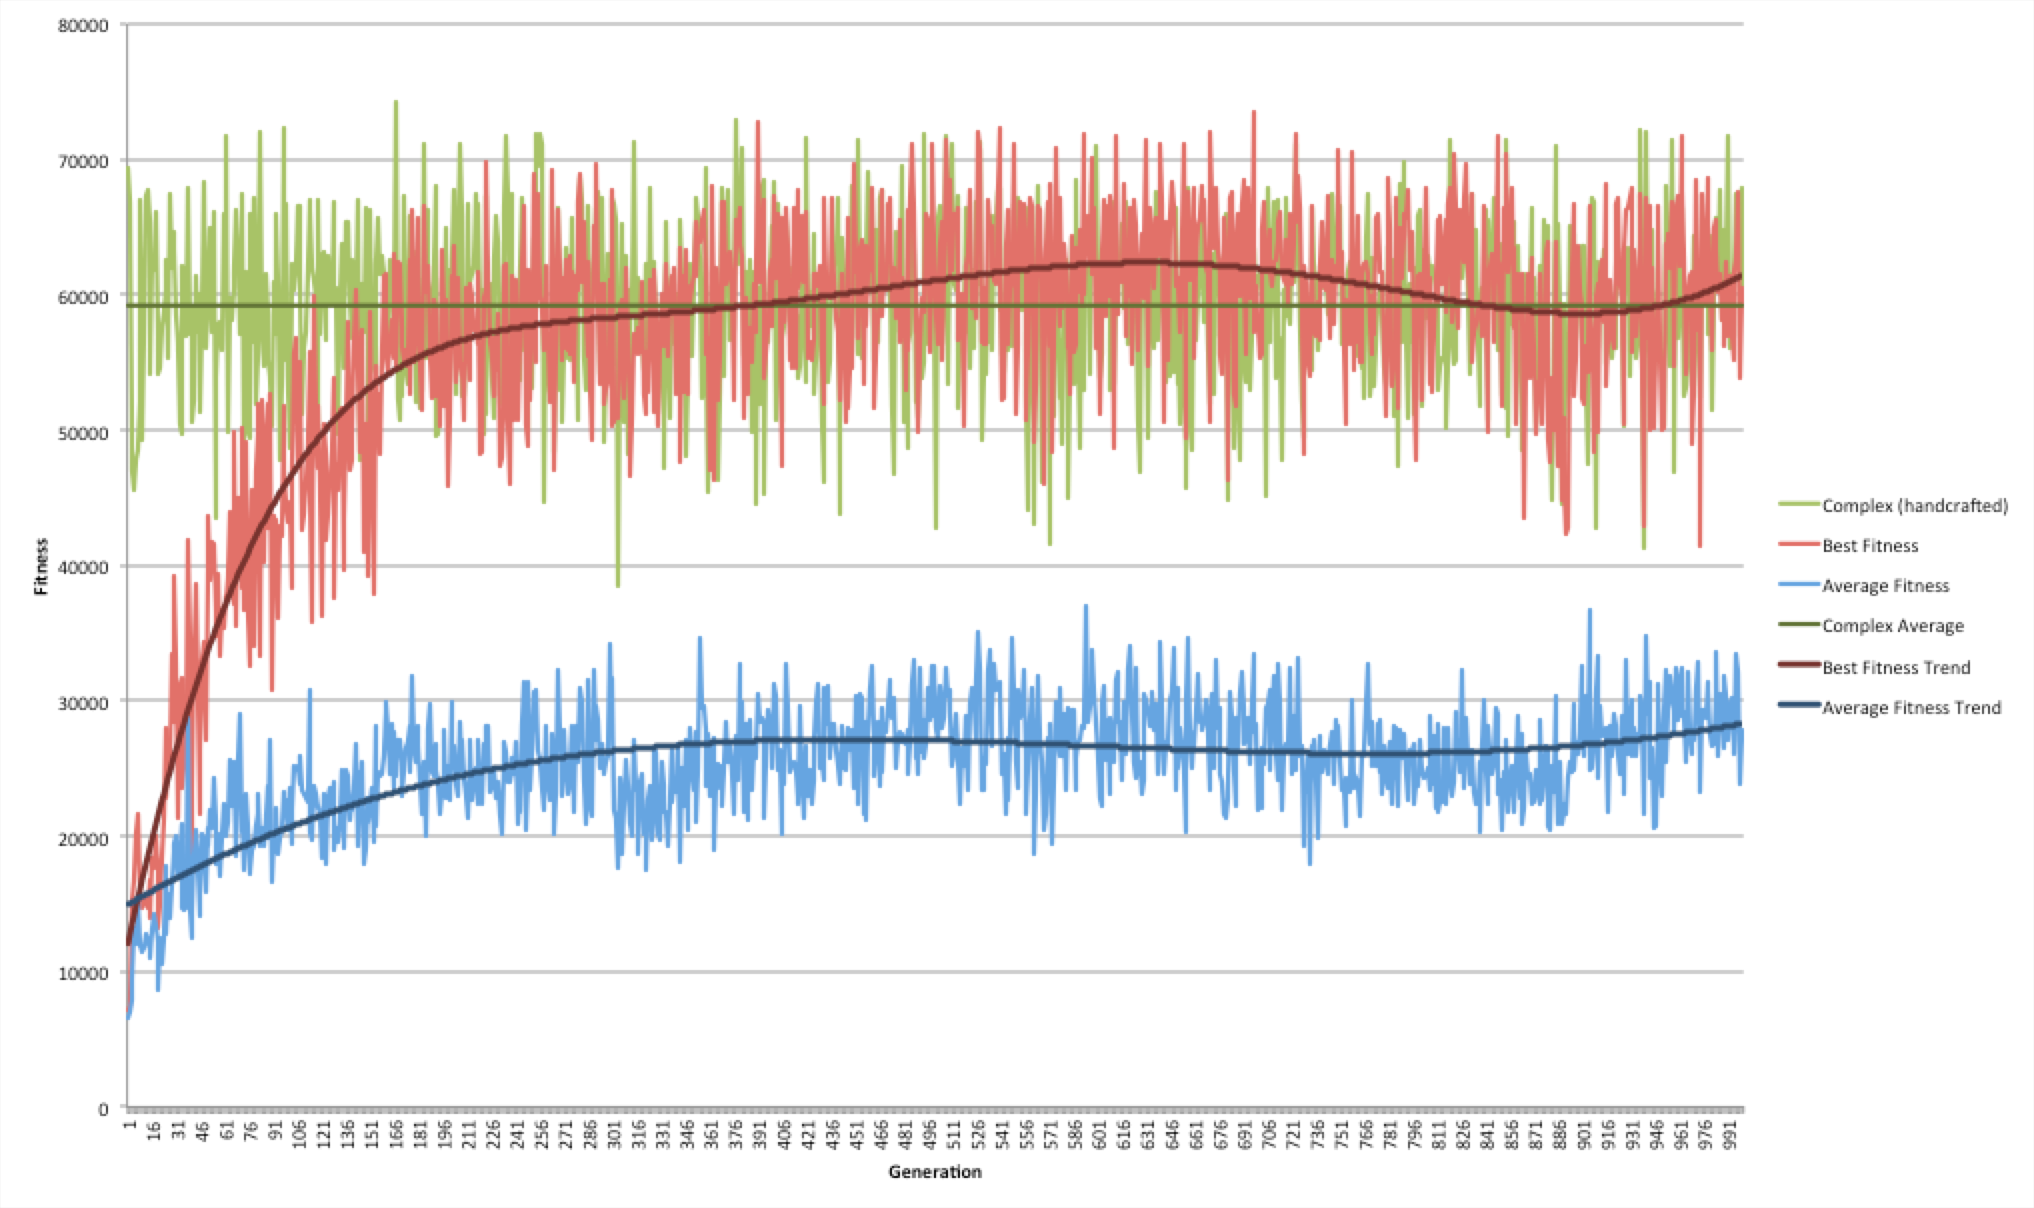
\includegraphics[scale=0.6]{LearnGraph.png}
  \caption{Graph charting the best and average fitness over the LEMMEL learning run. Handcrafted \textbf{complex} agent fitness also included.}
  \label{fig:learngraph}
 \end{figure}
\end{landscape}
}

Statistical output from each generation of the LEMMEL run (the most significant and successful learning run, described in Section \ref{subsec:learnparam}) was collated and organised. The information is presented in graphical form in Figure \ref{fig:learngraph}. It includes the best (red) and average (blue) fitness for each generation, with polynomial trend lines. The \textbf{complex} handcrafted agent (see Section \ref{subsec:hca}) was also passed into the evaluation task of each generation. Its fitness is also included on the graph in green.

\subsubsection{Improvement over Time}

From the graph we can see that both best and average fitness of the learning agents improved over time. Average fitness increased gently over the first 150 generations, from below 10,000 to around 25,000, after which it levelled off, with some fluctuations. Best fitness increase rapidly over the first 150 generations, from around 15,000 up to just below 60,000. It then rose more gently until generation 500, reaching around the 62,000 mark. There was a slight dip in best fitness after generation 850, which is likely explained by the high variance, which is explained in the the two proceeded sections.

The stagnation in improvement can be explained, in part, by the best individuals saturating the evaluation task. Scores above 60,000 are typical of very capable agent, ones who have completed 8 or 9 out of the 10 task levels. Scores over 70,000 represent a near perfect execution of the levels, completing them all in good time without many enemy collisions. We can see that, after generation 400, many populations contained individuals scoring in excess of 60,000, thus reducing the amount with which they could improve.

This is also reiterated by comparing the learnt agents' fitness with that of the complex agent. The trend line shows that the best performing agent of a generation often outperformed the handcrafted agent. Further analysis comparing the handcrafted agents with the those developed in the LEMMEL run is discussed in Section \ref{subsec:evallearnt}.


\subsubsection{Generation Variance}

A feature very evident in the LEMMEL graph is the amount of fitness variance between successive generations, which can be seen in both the best and average fitness. Analysis of the polynomial regressions reveals the standard error of regression for these datasets is 5,612 and 3,287 respectively. These figures are high for an optimisation algorithm, especially given that truncation selection usually helps to reduce deviation \cite[s.~3.8.3]{geatbx}. Moreover, as $\pmb{(\mu  + \lambda)}$ evolutionary strategy is being used (i.e. the best performing individuals are carried over to the next generation), one would not expect the best fitness to decrease very often. However, the data shows this occurs regularly.

This trait is due to the use of different level seed per generation, which means that each generation has a slightly different evaluation task. It was not expected that level seed would affect task difficulty (and therefore best fitness) as drastically as the data suggests.

To investigate this further, and to ascertain if it had any effect on the capability of the learn agent(s), a supplementary learning run was performed. This run had a single level seed, which was used in every generation, thus every generation had an identical evaluation task. For clarity, this run will be referred to as the \textbf{fixed-seed} run. The data from the fixed-seed run is charted in Figure \ref{fig:fixgraph}.

\afterpage{
\begin{landscape}
\begin{figure}
	\centering
	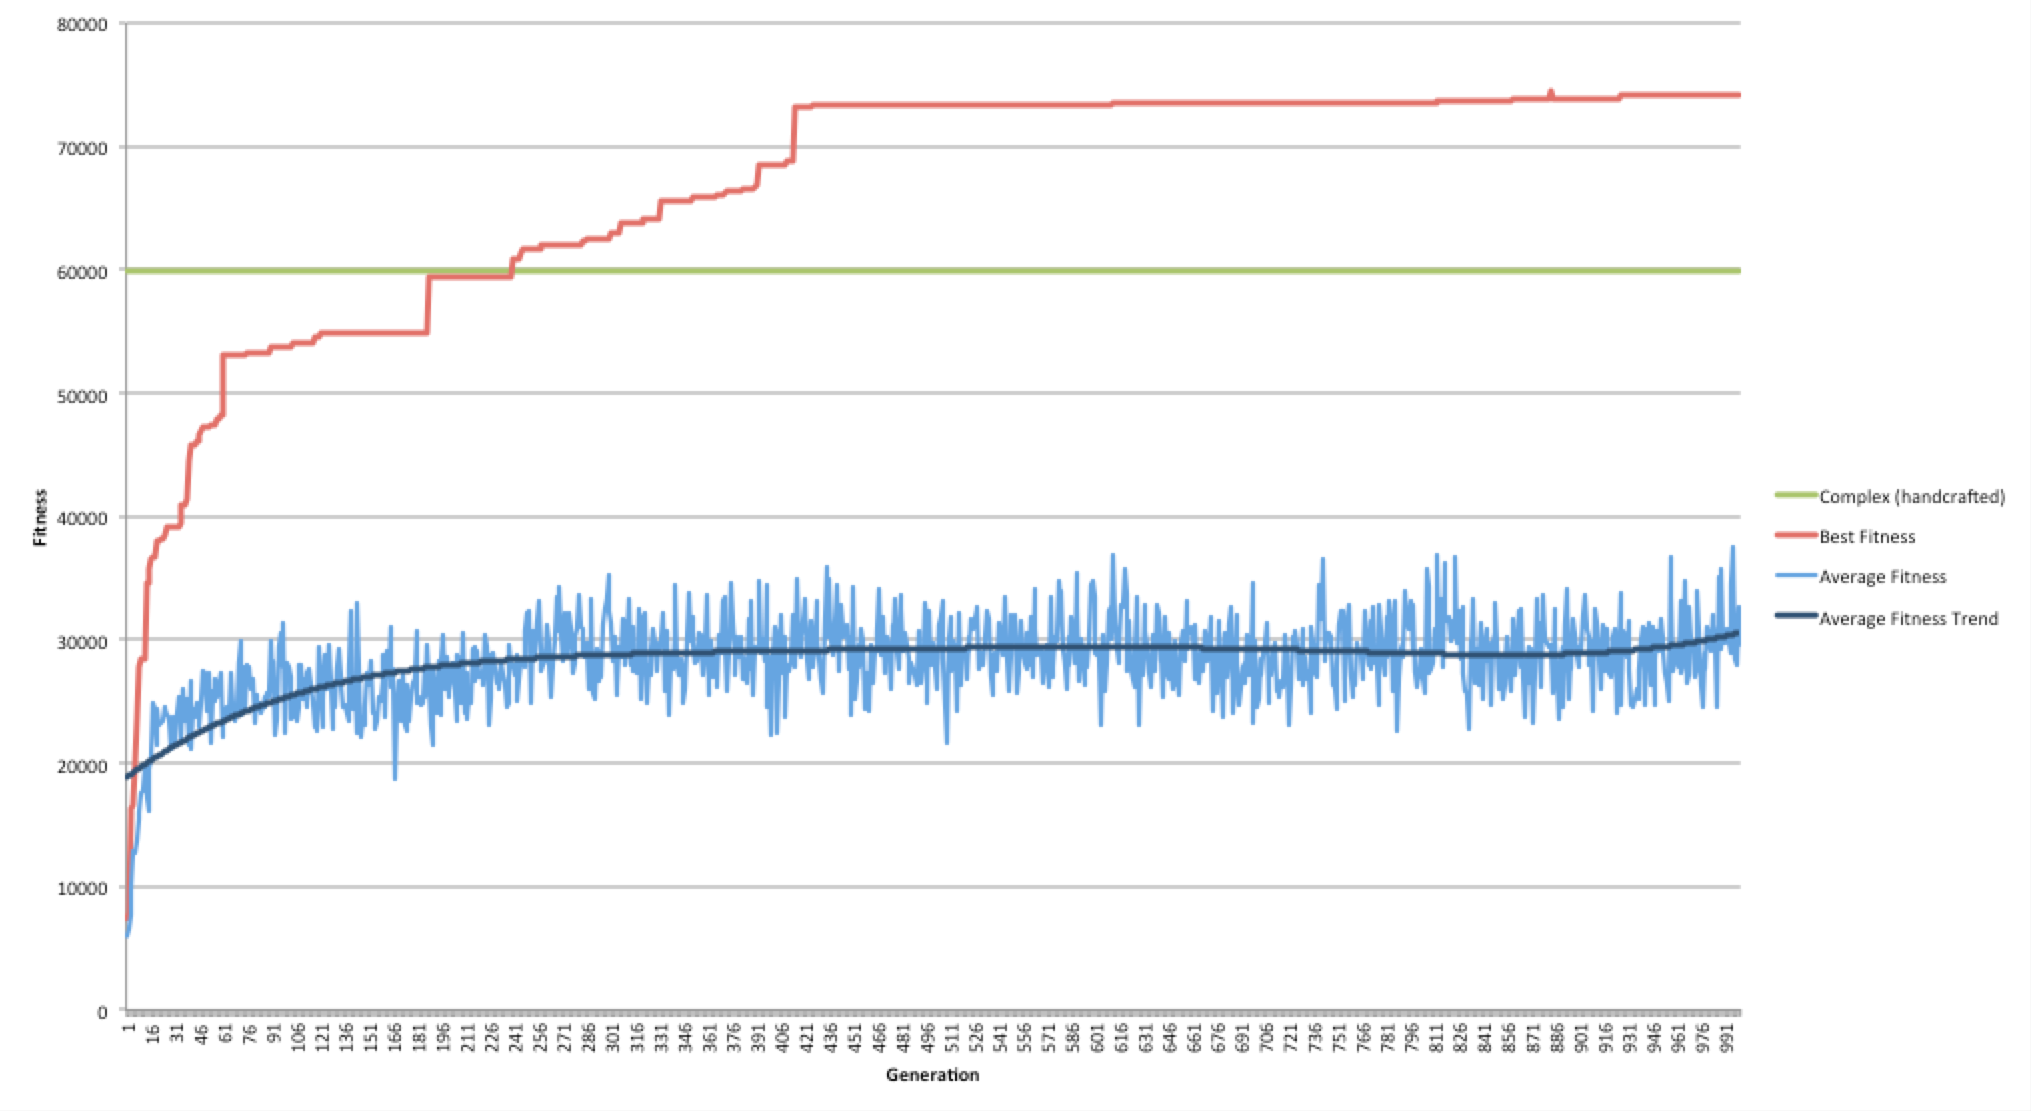
\includegraphics[scale=0.6]{FixSeedGraph.png}
	\caption{A learning run which had a fixed level seed, performed in response to high generational variation in the LEMMEL run.}
	\label{fig:fixgraph}
\end{figure}
\end{landscape}
}

As expected, the best fitness in this run only ever increased\footnote{Except for after generation 882. This fitness evaluation is erroneous and an example of the occasional non-deterministic nature of the benchmark game-engine. Attempts to repeat the value (using that generations best agent) were unsuccessful and instead produced a value that was lower than the previous generations best fitness.}. Moreoever, the deviation in average fitness decreased, with a standard error of regression of 2,817. Furthermore, the highest fitness achieved was higher, which may mean either it is more capable than those evolved in the LEMMEL run or simply became very suited to the fixed set of levels. To determine this the agent will be included in the learnt agent analysis in Section \ref{subsec:evallearnt}, alongside those from the LEMMEL run.

\subsubsection{Population Variance}

\begin{table}
  \begin{adjustwidth}{-0cm}{-0cm}
  \begin{center} \small
    \begin{tabular}{ | l | c | c |}
    \hline
    & \textbf{Average} & \textbf{Standard} \Tstrut \\
    \textbf{Run} & \textbf{Fitness} & \textbf{Deviation}  \Bstrut \\ \thickhline
    
    \textbf{LEMMEL} & 27,740 & 18,850 \\ \hline
    \textbf{Fixed Seed} & 29,601 & 25,293 \\ \hline
    
    \end{tabular}
  \end{center}
  \end{adjustwidth}
  \caption{\small Deviation over the fitness of the final population of the learning runs, demonstrating high population variance.}
  \label{tab:popvar}
\end{table}

Both the LEMMEL graph and the fixed seed graph show a large difference between best and average fitness. this suggests a high deviation over fitness within each population. This is confirmed by analysing the final generation of both runs, for which the full population statistics are available. The average fitness and standard deviation are shown in Table \ref{tab:popvar}.

As each generation is comprised entirely of children of the best individuals of the previous generation, such population variance shows that the ruleset genomes are highly sensitive to mutation. For example, we can consider the final population from the fixed seed run. The truncation selection of generation 999 restricted the parent pool to 5 individuals, each with a fitness of over 74,000. The generation 1000 population was made up entirely of their mutations, but still contained 23 (46\%) individuals whose fitness was under 10,000. 

More specifically, the best individual of generation 999 contained the following rule (a key for which can be found in Appendix \ref{app:percond}):

\begin{table}[!h]
  \begin{adjustwidth}{-2cm}{-2cm}
  \begin{center} \scriptsize
    \begin{tabular}{| c | c | c | c | c || c | c | c | c |}
    \hline
    \multirow{2}{*}{\textbf{\#}} & \multicolumn{4}{c ||}{\textbf{Conditions}} & \multicolumn{4}{c |}{\textbf{Actions}} \Tstrut \\ \cline{2-9}
	& \tiny ELR & \tiny OA & \tiny PB & \tiny MY & \tiny Left~ & \tiny Right & \tiny Jump~ & \tiny Speed \TBstrut \\ \thickhline
	15 & 0 & 0 & 0 & 1 	& F & F & F & F \\ \hline
    \end{tabular}
  \end{center}
  \end{adjustwidth}
\end{table}

This rule states that when there are no enemies or obstacles in front and no pit below, Mario should do nothing. The was rarely used due to the condition that Mario must also be moving down: \textbf{MY} (MovingY) = 1. In one individual, a single gene mutation removed the condition on \textbf{MY}, this caused the rule to activate constantly at the beginning of each level, leaving Mario frozen. This caused the fitness to drop from 74,194 to 4,687, which shows that a single mutation can have a devastating affect on ruleset fitness.

%-----------------------------------------------------------------------
% Learnt Agents
%-----------------------------------------------------------------------

\subsection{Handcrafted vs. Learnt Agents}
\label{subsec:evallearnt}

As explained in Section \ref{subsec:learnstats}, the learning process was configured to extract three rulesets to be considered for evaluation. After generation 800, the algorithm saves the agent with the best overall fitness and the agent with the largest fitness compared to the average. The two such agents from the LEMMEL run (alongside the final agent from the fixed seed run) are compared to the handcrafted agents in this section. For reference, they will be named \textbf{learnt best}, \textbf{learnt difference} and \textbf{learnt fixed seed} agents respectively, and called the learnt agents collectively.

\subsubsection{Learning Evaluation Task}

\begin{table}[t]
  \begin{adjustwidth}{-0cm}{-0cm}
  \begin{center} \small
    \begin{tabular}{ | l | c | c | c | c |}
    \hline
    \textbf{Agent} & \textbf{Average} & \textbf{Offset} & \textbf{Best} & \textbf{Worst} \TBstrut \\ \thickhline
    \textbf{Complex} & 59,206 & 0 & 74,286 & 38,494  \\ \hline
    \textbf{Simple Reactive} & 37,310 & 21,896 & 61,784 & 19,526 \\ \hline
    \textbf{Forward Jumping} & 20,458 & 38,748 & 45,022 & 8,378 \\ \thickhline
    \textbf{Learnt Difference} & 58,930 & 276 & 72,672 & 36,440  \\ \hline
    \textbf{Learnt Best} & 59,079 & 127 & 73,058 & 43,740  \\ \hline
    \textbf{Learnt Fixed Seed} & 54,115 & 5,091 & 74,194 & 38,494  \\ \hline
    \end{tabular}
  \end{center}
  \end{adjustwidth}
  \caption{\small Statistics from handcrafted and learnt agents playing each generation's evaluation task from the LEMMEL run.}
  \label{tab:learnrunagents}
\end{table}

The three learnt agents and three handcrafted agents were run through the each generation's evaluation task of the LEMMEL run. The agents perfrom 1000 tasks, with the options and level seed from LEMMEL parameter file (full details can be found in Section \ref{subsec:learnparam}. Results are compiled in to Table\ref{tab:learnrunagents}. We can see from the data that both the leant best and learnt difference agents performed at the same level as the complex agent and considerable better than the other handcrafted agents. Which implies they became very capable at the task they were learning on. This is especially significant as the LEMMEL evaluation task was designed to favour the complex and simple reactive agents.

We can also see that the learnt fixed seed agent did not perform quite as well, suggesting it became too suited to the single set of levels it was evolved over. The large difference between best and worst fitness for each agent reiterates that the use of different level seeds may be overly affecting difficulty. However, as the learnt fixed seed agent did not score as highly as the other learnt agents, it suggests that although the LEMMEL run had high generational variance, it produced more capable agents.

\subsubsection{Comparator Task}

\begin{table}
  \begin{adjustwidth}{-0cm}{-0cm}
  \begin{center} \small
    \begin{tabular}{ | l | c | c | c | c | c |}
    \hline
    & \textbf{Total} & \textbf{Levels} & \textbf{Enemies} & \Tstrut \\
    \textbf{Agent} & \textbf{Score} & \textbf{Completed} & \textbf{Killed} & \textbf{Distance} \Bstrut \\ \thickhline
    \textbf{Complex} & 1,758,931 & 168 (33\%) & 1,440 (8\%) & 62,231 (45\%) \\ \hline
    \textbf{Simple Reactive} & 1,102,733 & 87 (17\%) & 588 (3\%) & 44,038 (32\%) \\ \hline
    \textbf{Forward Jumping} & 954,141 & 65 (13\%) & 743 (4\%) & 38,484 (28\%) \\ \thickhline
    \textbf{Learnt Difference} & 1,521,200 & 144 (28\%) & 1,130 (6\%) & 55,710 (40\%) \\ \hline
    \textbf{Learnt Best} & 1,510,697 & 133 (26\%) & 1,603 (8\%) & 54,341 (39\%) \\ \hline
    \textbf{Learnt Fixed Seed} & 1,267,914 & 102 (20\%) & 1,173 (6\%) & 48,131 (35\%) \\ \hline
    \end{tabular}
  \end{center}
  \end{adjustwidth}
  \caption{\small Competitive statistics from handcrafted and learnt agents playing the comparator task with a seed of 1000.}
  \label{tab:learnagentcomp}
\end{table}

The six agents were also passed into the more extensive comparator task (described in Section \ref{subsec:comptask}) with a seed of 1000. Each agents results are presented in Table \ref{tab:learnagentcomp}. We can see from the data that both the Leant best and Learnt difference agents performed better than the two simpler handcrafted agents, but not as well as the complex agent. Considering the evaluation task result, this shows that the learning evaluation task may not adequately represent the comparator task and the game more generally. We can also see that the learnt fixed seed agent did not perform quite as well, suggesting that agents that learn from many sets of levels are more adept at tackling a greater variety of challenges.

Figure \ref{fig:compgraph} shows how the agents performed at different difficulties in the comparator task. None of the agents performed well on difficulties over 10. Further analysis showed that they all failed to clear the large jumps which are common to these levels, demonstrating a weakness in the agent framework. Elsewhere, the complex agent outperformed the learnt agents on nearly all difficulties. However, both the learnt best and the learnt difference agents did outperform it on difficulty 2 .This was the most prevalent difficulty in the LEMMEL evaluation task and suggests that a longer or more representative task may produce a more capable agent. We can also see that the disparity between the learnt fixed seed agent and its peers come mainly form the lower difficulty levels. At these difficulties the other learnt agents take greater advantage of the reduced presence of enemies and pits. This is especially true of difficulty 0, in which there are no pits and very simple enemies, where the fixed seed agent was outperformed by all the other agents.


\afterpage{
\begin{landscape}
 \begin{figure}
  \centering
  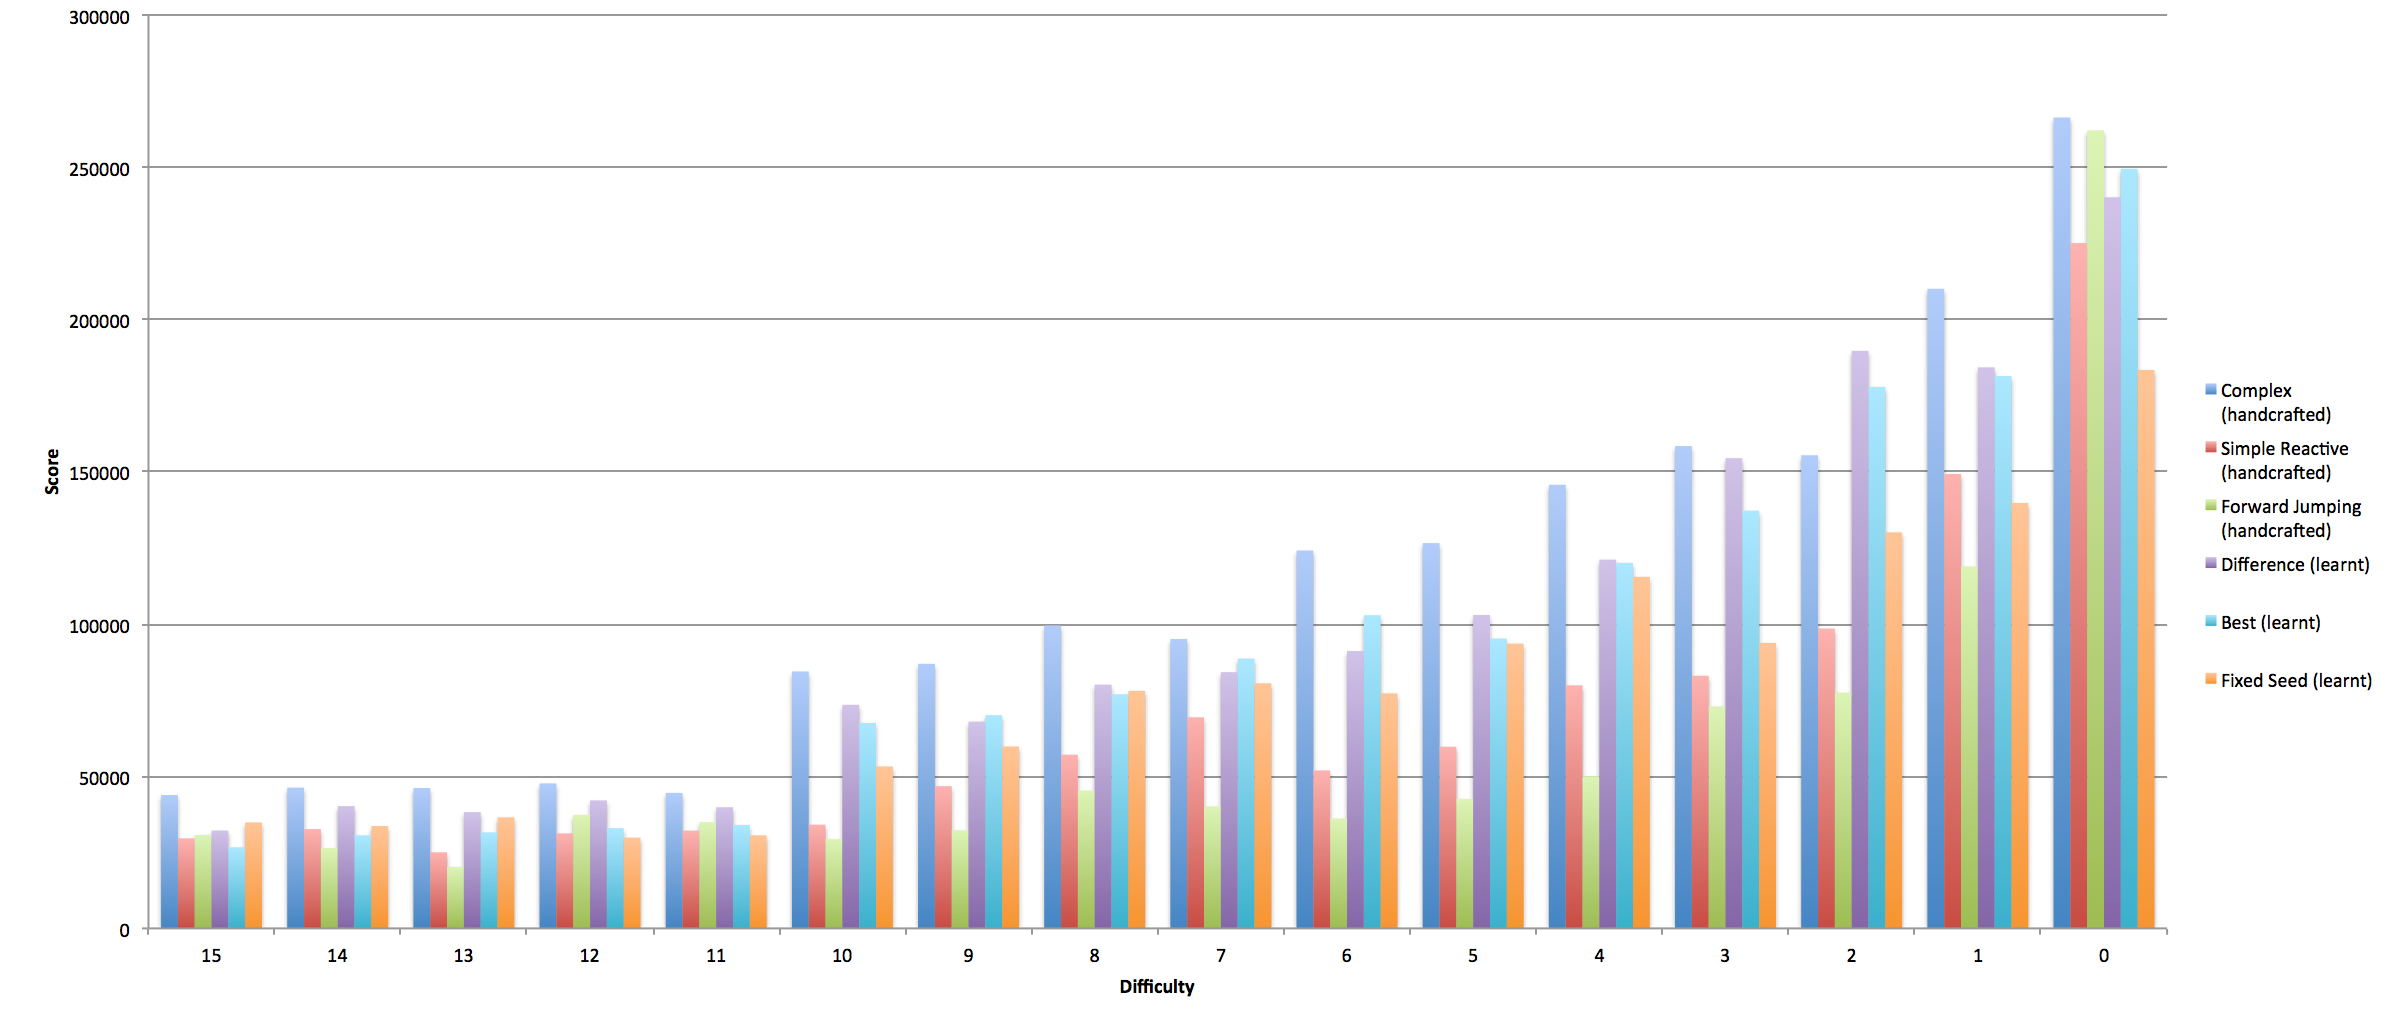
\includegraphics[scale=0.5]{CompTaskGraph.png}
  \caption{Graph charting the score achieved on different difficulty levels during the comparator task.}
  \label{fig:compgraph}
 \end{figure}
\end{landscape}
}

%-----------------------------------------------------------------------
% Learnt Agent Behaviours
%-----------------------------------------------------------------------
\subsection{Learnt Agent Analysis}
\label{subsec:evallearn2}


\begin{table}[!t]
  \begin{adjustwidth}{-2cm}{-2cm}
  \begin{center} \scriptsize
    \begin{tabular}{ | c | c | c | c | c | c | c | c | c | c | c | c || c | c | c | c |}
    \hline
    \multirow{2}{*}{\textbf{\#}} & \multicolumn{11}{c ||}{\textbf{Conditions}} & \multicolumn{4}{c |}{\textbf{Actions}} \Tstrut \\ \cline{2-16}
    
	& \tiny MM & \tiny JA & \tiny OG & \tiny EL & \tiny EUR & \tiny ELR & \tiny OA & \tiny PA & \tiny PB & \tiny MX & \tiny MY & \tiny Left~ & \tiny Right & \tiny Jump~ & \tiny Speed \TBstrut \\ \thickhline
	1 & & & 1 & & 1 & 1 & & 0 & 1 & 2 & 0 		& & & T & T \\ \hline
	2 & & 0 & & & & & & & & 2 & 2		& & T & T & T \\ \hline
	3 & & 1 & & & 1 & & 1 & & 0 & & 0 		& & & T & T \\ \hline
	4 & & 0 & 0 & & & 0 & 1 & 0 & 1 & 0 & 1 		& T & T & T & T \\ \hline
	5 & & & & & 0 & 0 & 1 & & 0 & 0 & 0 		& & & T & \\ \hline
	6 & & 0 & & & 1 & 1 & 1 & & 0 & 0 & 		& & & T & T \\ \hline
	7 & & 1 & 0 & & & 0 & & 0 & 0 & & 2 		& & & & \\ \hline
	8 & & & & 0 & 0 & 0 & 0 & & 1 & 2 & 1		& & T & T & T \\ \hline
	9 & & & & & & & & & 0 & 0 & 2 		& & & T & \\ \hline
	10 & & 0 & 1 & & & & 1 & 1 & & 0 & 		& & & & \\ \hline
	11 & 0 & & 1 & 1 & 0 & 1 & & 1 & 0 & & 1 		& & T & & T \\ \hline
	12 & & & & & 1 & & & 2 & & & 		& & & & T \\ \hline
	13 & & & & & & & 0 & & 0 & 2 & 1 		& T & & T & T \\ \hline
	14 & & 1 & 0 & 1 & 0 & 1 & 1 & 0 & & 0 & 		& T & T & T & T \\ \hline
	15 & & 1 & & & & & & & 1 & 0 & 2 		& T & T & T & T \\ \hline
	16 & & 1 & 1 & 0 & & & & 1 & & & 		& T & T & T & \\ \hline
	17 & & 1 & 1 & & 0 & & & & 1 & & 0 		& & T & T & T \\ \hline
	18 & & 1 & 1 & & & 1 & & 0 & & & 		& & & T & \\ \hline
	19 & & 1 & & & 1 & & & 2 & 0 & & 0 		& T & & & T \\ \hline
	20 & & & 0 & & & 0 & 0 & & 0 & 0 & 0 		& T & T & T & T \\ \hline
		
	-  & & & & & & & & & & & 		& & T & & T \\ \hline
    \end{tabular}
  \end{center}
  \end{adjustwidth}
  \caption{Ruleset for learnt difference agent. Blank entries denote {\scriptsize DONT\_CARE} for Conditions and \textbf{false} for Actions. A key for this table can be found in Appendix \ref{app:percond}}
  \label{tab:LDA}
\end{table}

Of all the learnt agents, the learnt difference agent performs the best on the comparator task. It also demonstrates the most interesting behaviour, which is analysed in this section. A full ruleset for this agent can be found in Table \ref{tab:LDA}, a key for the table can be found in Appendix \ref{app:percond}.

\subsubsection{Rule usage}

The agent only regularly uses 7 of its 20 rules (35\%), and relies heavily on the default action. On one hand, some of its rules contain conditions that are too specific, for example, Rule 11, which is never used. On the other, some rules are not specific enough and are eclipsed by others, for example, Rule 12, which is often forgone in favour of Rule 19. Rather than mutation or favour rate (see Section \ref{subsec:learndes}) being too high or too low, this suggests that the design of the genome mutation itself is too simplistic. Methods of addressing this are discussed in the Section \ref{subsec:evallearn}.

\subsubsection{Behaviours}

The learnt difference agent acts similarly to the complex and simple reactive agents; it attempts to jump over obstacles, pits and enemies when it detects them and runs at speed otherwise. It struggles with the largest pits and avoiding collisions when enemy concentration is high. Moreover, much like the complex agent, it occasionally gets stuck in an action loop and runs out of time.

Four significant and interesting behaviours and the rules that enable them are presented subsequently. 


\subsubsection*{Enemies}

\begin{table}[!h]
  \begin{adjustwidth}{-2cm}{-2cm}
  \begin{center} \scriptsize
    \begin{tabular}{| c | c | c | c | c | c | c | c | c || c | c | c | c |}
    \hline
    \multirow{2}{*}{\textbf{\#}} & \multicolumn{8}{c ||}{\textbf{Conditions}} & \multicolumn{4}{c |}{\textbf{Actions}} \Tstrut \\ \cline{2-13}
	& \tiny JA & \tiny OG & \tiny ELR & \tiny OA & \tiny PA & \tiny PB & \tiny MX & \tiny MY & \tiny Left~ & \tiny Right & \tiny Jump~ & \tiny Speed \TBstrut \\ \thickhline
	2 & 0 & & & & & & 2 & 2 &    F & T & T & T \\ \hline
	13 & & & & 0 & & 0 & 2 & 1 &    T & F & T & T \\ \hline
	18 & 1 & 1 & 1 & & 0 & & & &    F & F & T & F \\ \hline
	- &  & & & &  &  &  &  &    F & T & F & T \\ \hline
    \end{tabular}
  \end{center}
  \end{adjustwidth}
\end{table}

To avoid colliding with enemies the agent uses Rules 2, 13 and 18, together with the the default action. These rules are pictured above with the final entry denoting the default action/rule. A key for these rules can be found in Appendix \ref{app:percond}.

Figure \ref{fig:laej} illustrates this behaviour. Mario approaches the enemy using the default action. On detecting the enemy (\textbf{ELR} (EnemyLowerRight) = 1) Rule 18 activates and Mario jumps. Mario is now travelling up and right (\textbf{MX} (MovingX) = 2, \textbf{MY} (MovingY) = 2), thus Rule 2 activates to continue the jump and move him quickly to the right. Rule 2 also has the side effect of shooting a fireball if Mario is in \textbf{fire} mode. Rule 13 activates as Mario starts to descend (\textbf{MY} = 1), turning Mario left and slowing the jump. This allows the fireball to beat Mario to the landing zone, killing any enemies that might pose an immediate threat.

Enemy avoidance is the weakness of several of the learnt agents. The difference agent's approach of jumping high over them and shooting a fireball is one of the most effective. Using Rule 13 to slow the jump once the enemy is cleared allows Mario to avoid jumping into subsequent enemies or pits.

\begin{figure}[t]
	\begin{adjustwidth}{-2cm}{-2cm}
    \centering
          \begin{subfigure}[b]{0.49\textwidth}
                  \centering
                  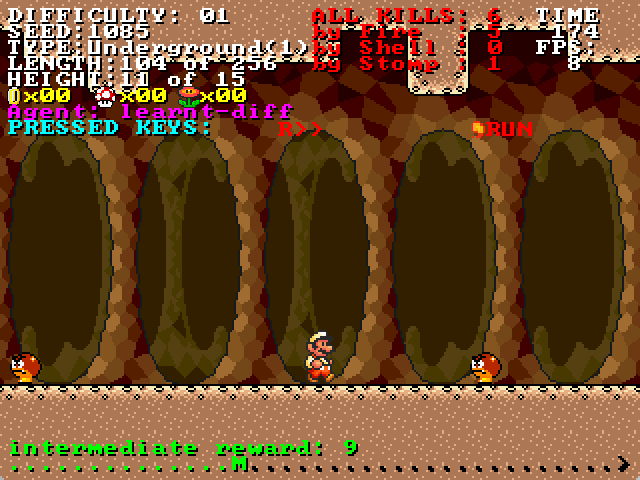
\includegraphics[width=\textwidth]{laej1.png}
                  \caption{Default Rule}
                  \vspace*{\baselineskip}
          \end{subfigure}~
          \begin{subfigure}[b]{0.49\textwidth}
                  \centering
                  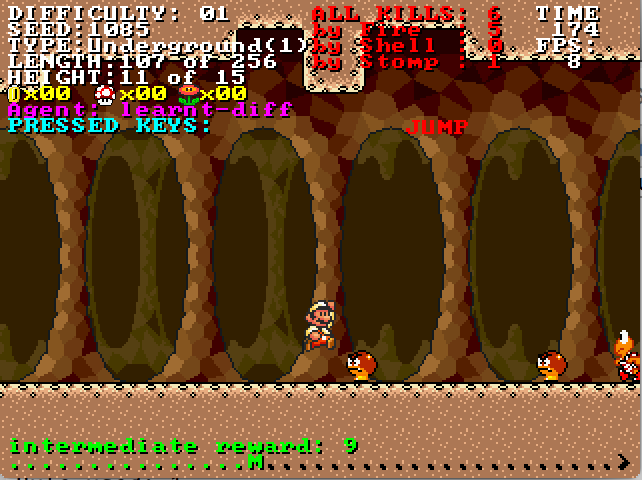
\includegraphics[width=\textwidth]{laej2.png}
                  \caption{Rule 18}
                  \vspace*{\baselineskip}
          \end{subfigure}
          \begin{subfigure}[b]{0.49\textwidth}
                  \centering
                  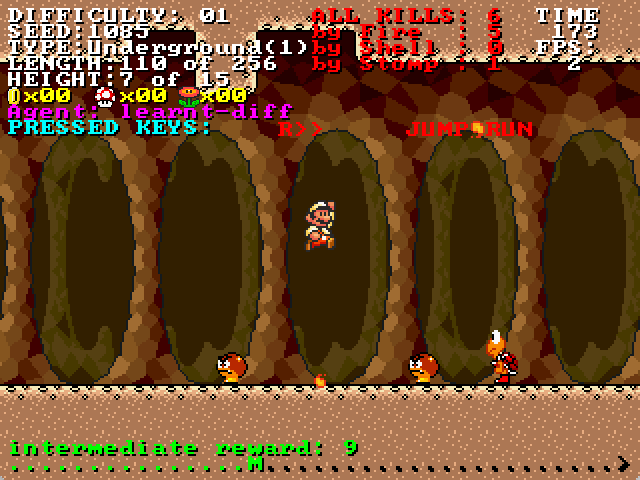
\includegraphics[width=\textwidth]{laej3.png}
                  \caption{Rule 2}
                  \vspace*{\baselineskip}
          \end{subfigure}~
          \begin{subfigure}[b]{0.49\textwidth}
                  \centering
                  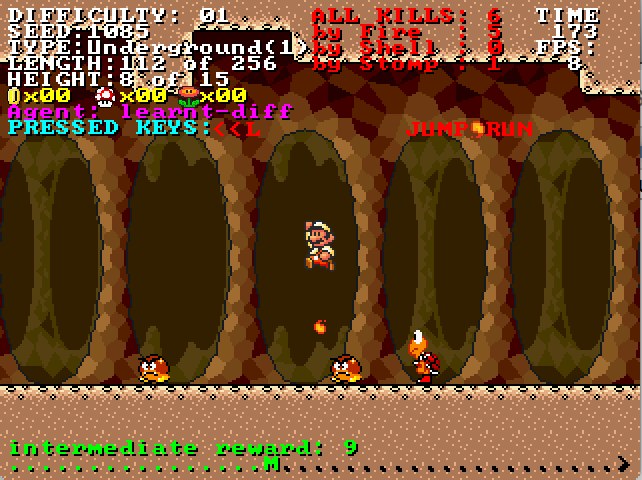
\includegraphics[width=\textwidth]{laej4.png}
                  \caption{Rule 13}
                  \vspace*{\baselineskip}
          \end{subfigure}
          \begin{subfigure}[b]{0.49\textwidth}
                  \centering
                  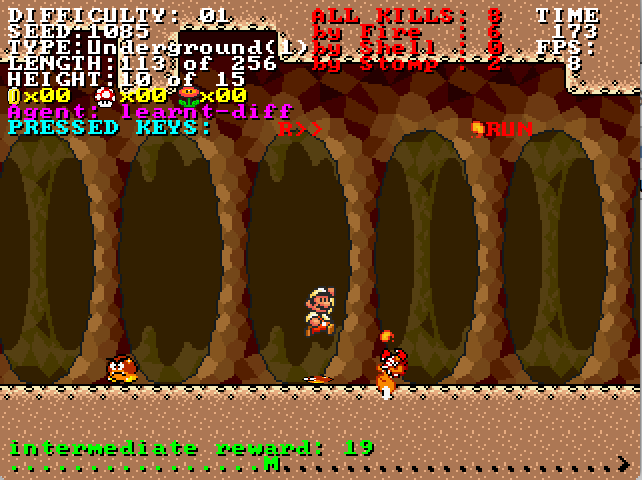
\includegraphics[width=\textwidth]{laej5.png}
                  \caption{Default Rule}
                  \vspace*{\baselineskip}
          \end{subfigure}~
          \begin{subfigure}[b]{0.49\textwidth}
                  \centering
                  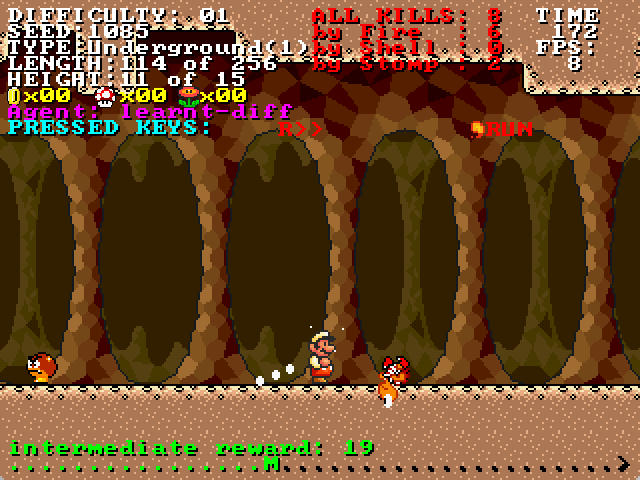
\includegraphics[width=\textwidth]{laej6.png}
                  \caption{Default Rule}
                  \vspace*{\baselineskip}
          \end{subfigure}
    \caption{Learnt Difference agent tackling enemies.}\label{fig:laej}
    \end{adjustwidth}
\end{figure}


\clearpage
%\vspace*{\stretch{2}}
\vspace*{\baselineskip}
\subsubsection*{Obstacles}

\begin{table}[!h]
  \begin{adjustwidth}{-2cm}{-2cm}
  \begin{center} \scriptsize
    \begin{tabular}{| c | c | c | c | c | c | c || c | c | c | c |}
    \hline
    \multirow{2}{*}{\textbf{\#}} & \multicolumn{6}{c ||}{\textbf{Conditions}} & \multicolumn{4}{c |}{\textbf{Actions}} \Tstrut \\ \cline{2-11}
	& \tiny EUR & \tiny ELR & \tiny OA & \tiny PB & \tiny MX & \tiny MY & \tiny Left~ & \tiny Right & \tiny Jump~ & \tiny Speed \TBstrut \\ \thickhline
	5 & 0 & 0 & 1 & 0 & 0 & 0 &    F & F & T & F \\ \hline
	9 & & & & 0 & 0 & 2 &    F & F & T & F \\ \hline
	13 & & & 0 & 0 & 2 & 1 &    T & F & T & T \\ \hline
	- &  &  &  &  &  &  &    F & T & F & T \\ \hline
    \end{tabular}
  \end{center}
  \end{adjustwidth}
\end{table}

In order to overcome obstacles, such as level terrain and blocks, the agent uses Rules 5 and 9, in conjunciton with the default action.

The process is demonstrated in Figure \ref{fig:laob}. The agent approaches the wall using the default action. On hitting the obstruction, Mario stops moving (\textbf{MX} (MovingX) = 0, \textbf{MY} (MovingY) = 0) and detects the obstacle (\textbf{OA} (ObstacleAhead) = 1). This activates Rule 5, causing Mario to jump. As Mario is now moving straight upwards (\textbf{MX} = 0, \textbf{MY} = 2) Rule 9 is activate and ensures Mario continues the jump to its maximum height. When descending, Mario alternates between using Rule 13 and the default action. This results in Mario moving slightly to the right and landing on the obstacle, successfully clearing it.

The behaviour is particularly interesting due to the condition on Mario being stationary before jumping. This allows Mario to clear obstacles without over-jumping. Over-jumping could cause a him to fall into a proceeding pit, especially when climbing `stairs' (see Figure \ref{fig:lapj}).

This is an example of a behaviour not considered during the construction of the handcrafted agents. The complex agent handles the issue of over-jumping by detecting potential problems and moving left.

Many evolved rulesets, through several of the learning runs, demonstrate this behaviour, confirming its benefit to the agent. Furthermore, during the LEMMEL run, it is one of the earliest to develop, appear first at around generation 50.

%\vspace*{\stretch{3}}
\clearpage

\begin{figure}[m]
	\begin{adjustwidth}{-2cm}{-2cm}
    \centering
          \begin{subfigure}[b]{0.49\textwidth}
                  \centering
                  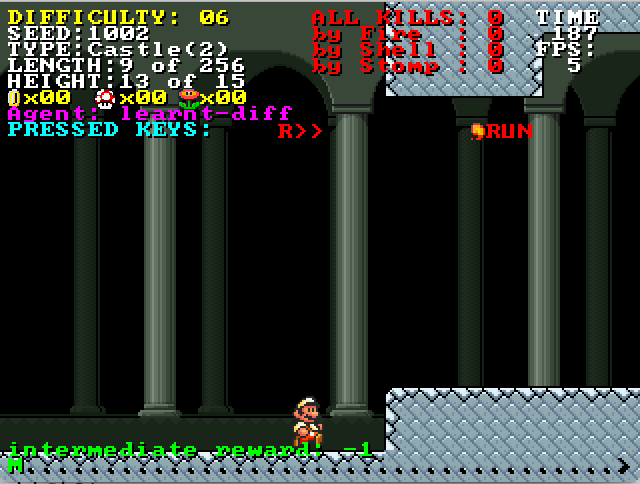
\includegraphics[width=\textwidth]{laob1.png}
                  \caption{Default Rule}
                  \vspace*{\baselineskip}
          \end{subfigure}~
          \begin{subfigure}[b]{0.49\textwidth}
                  \centering
                  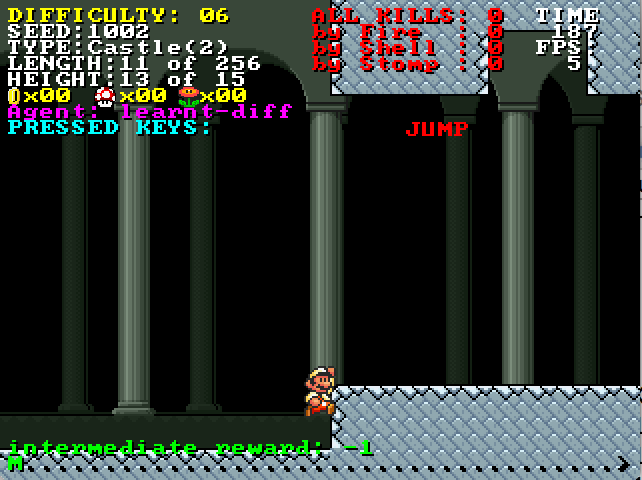
\includegraphics[width=\textwidth]{laob2.png}
                  \caption{Rule 5}
                  \vspace*{\baselineskip}
          \end{subfigure}
          \begin{subfigure}[b]{0.49\textwidth}
                  \centering
                  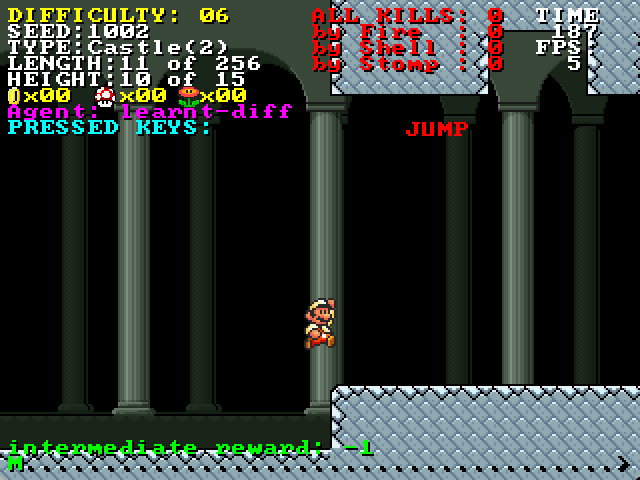
\includegraphics[width=\textwidth]{laob3.png}
                  \caption{Rule 9}
                  \vspace*{\baselineskip}
          \end{subfigure}~
          \begin{subfigure}[b]{0.49\textwidth}
                  \centering
                  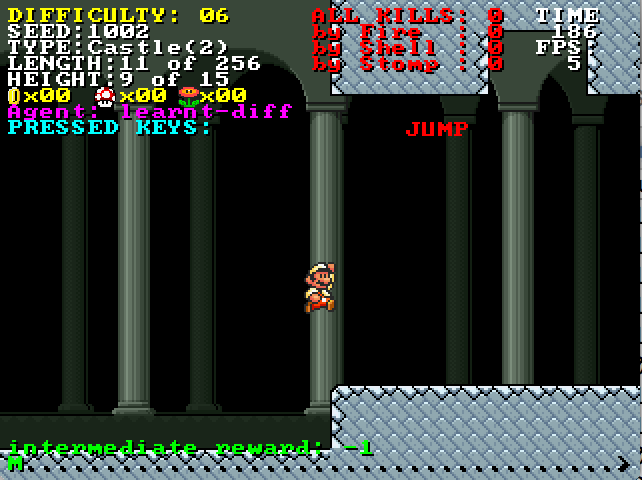
\includegraphics[width=\textwidth]{laob4.png}
                  \caption{Rule 9}
                  \vspace*{\baselineskip}
          \end{subfigure}
          \begin{subfigure}[b]{0.49\textwidth}
                  \centering
                  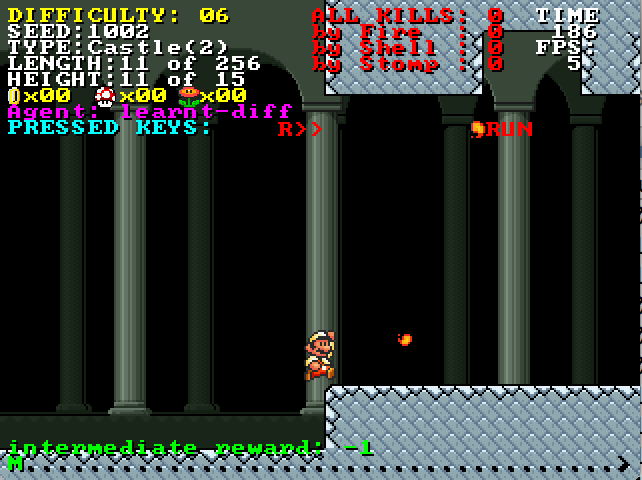
\includegraphics[width=\textwidth]{laob5.png}
                  \caption{Default Rule}
                  \vspace*{\baselineskip}
          \end{subfigure}~
          \begin{subfigure}[b]{0.49\textwidth}
                  \centering
                  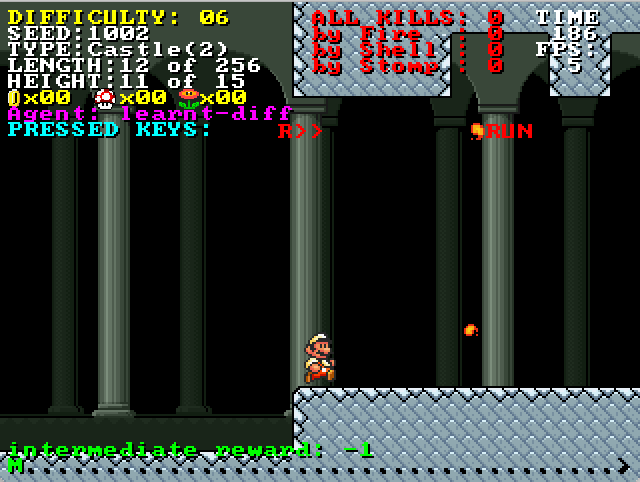
\includegraphics[width=\textwidth]{laob6.png}
                  \caption{Default Rule}
                  \vspace*{\baselineskip}
          \end{subfigure}
    \caption{Learnt Difference agent tackling obstacles, without over-jumping.}\label{fig:laob}
    \end{adjustwidth}
\end{figure}


\clearpage

\vspace*{\baselineskip}
\subsubsection*{Pits}

\begin{table}[!h]
  \begin{adjustwidth}{-2cm}{-2cm}
  \begin{center} \scriptsize
    \begin{tabular}{| c | c | c | c | c | c | c | c | c | c | c || c | c | c | c |}
    \hline
    \multirow{2}{*}{\textbf{\#}} & \multicolumn{10}{c ||}{\textbf{Conditions}} & \multicolumn{4}{c |}{\textbf{Actions}} \Tstrut \\ \cline{2-15}
	& \tiny JA & \tiny OG &  \tiny EL & \tiny EUR & \tiny ELR & \tiny OA & \tiny PA & \tiny PB & \tiny MX & \tiny MY & \tiny Left~ & \tiny Right & \tiny Jump~ & \tiny Speed \TBstrut \\ \thickhline
	2 & 0 & & & & & & & & 2 & 2 &    F & T & T & T \\ \hline
	8 & & & 0 & 0 & 0 & 0 & & 1 & 2 & 1 &      F & T & T & T \\ \hline
	13 & & & & & & 0 & & 0 & 2 & 1 &    T & F & T & T \\ \hline
	16 & 1 & 1 & 0 & & & & 1 & & & &    T & T & T & F \\ \hline
	- &  & & & &  & & &  &  &  &    F & T & F & T \\ \hline
    \end{tabular}
  \end{center}
  \end{adjustwidth}
\end{table}

To jump over pits Mario uses Rules 2, 8, 13 and 16, along with the default action.

Mario can be seen jumping over a pit with `stairs' in Figure \ref{fig:lapj}. If the pit does not have stairs then Mario approaches using the default action, otherwise, he climbs them one by one using his obstacle behaviour. As soon as he lands on the top step (\textbf{JA} (JumpAvailable) = 1, \textbf{OG} (OnGround) =1) he detects that the pit is close (\textbf{PA} (PitAhead) = 1). This activates Rule 16, causing Mario to jump. Rule 2 then activates to maximise the jump (as we saw with enemies). When Mario reaches the top of the jump and begins to descend (\textbf{MY} (MovingY) = 1) Rule 2 deactivates. If Mario is still above the pit (\textbf{PB} (PitBelow) = 1) Rule 8 is used to ensure Mario reaches as far as possible. As soon as Mario is no longer over the pit (\textbf{PB} = 0) Rule 13 is used to slow the jump and avoid over-jumping. If Rule 13 is used to the point that Mario stops moving right (\textbf{MX} (MovingX) = 0 or 1) the default action is used instead, which helps Mario avoid turning back into the pit. Often, this means that Mario lands the very edge of the pit, at which point he uses the default action to continue.

Pits are the most dangerous part of any level, as they can cause an instant loss. Hence, clearing them is vitally important for the capability of an agent. The learnt agent's strategy of always maximise the jump whilst it is above a pit means that it clears the majority of them. Furthermore, its ability to just on the right-hand side of the pit allows Mario to successfully avoid over-jumping and tackle the next hurdle.

Every learnt agent displays some level of this behaviour. However, most of them are negatively affected by the proximity of enemies, whereas the learnt agent's pit strategy is less concerned with their presence. This is important as a pit can cause instant failure, whereas an enemy collision is only fatal when in \textbf{small} mode. In fact, the learnt agent also displays an additional positive behaviour in regards to the combination of enemies and pits, which is explained next.


\clearpage

\begin{figure}[m]
	\begin{adjustwidth}{-2cm}{-2cm}
    \centering
          \begin{subfigure}[b]{0.49\textwidth}
                  \centering
                  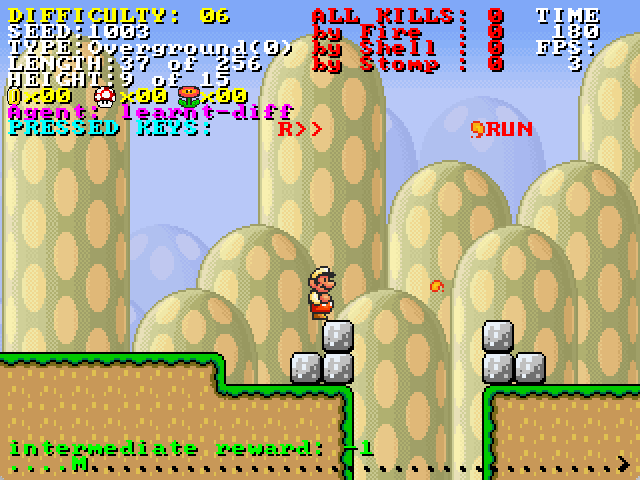
\includegraphics[width=\textwidth]{lapj1.png}
                  \caption{Default Rule}
                  \vspace*{\baselineskip}
          \end{subfigure}~
          \begin{subfigure}[b]{0.49\textwidth}
                  \centering
                  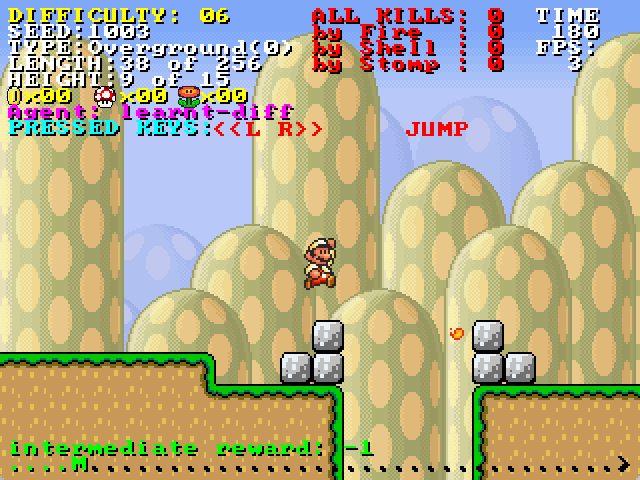
\includegraphics[width=\textwidth]{lapj2.png}
                  \caption{Rule 16}
                  \vspace*{\baselineskip}
          \end{subfigure}
          \begin{subfigure}[b]{0.49\textwidth}
                  \centering
                  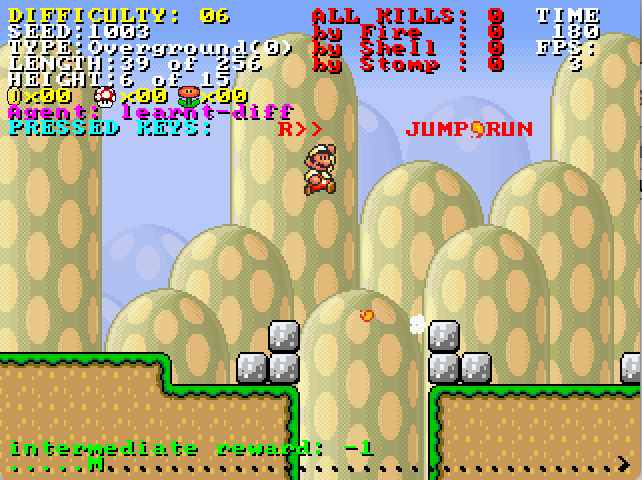
\includegraphics[width=\textwidth]{lapj3.png}
                  \caption{Rule 2}
                  \vspace*{\baselineskip}
          \end{subfigure}~
          \begin{subfigure}[b]{0.49\textwidth}
                  \centering
                  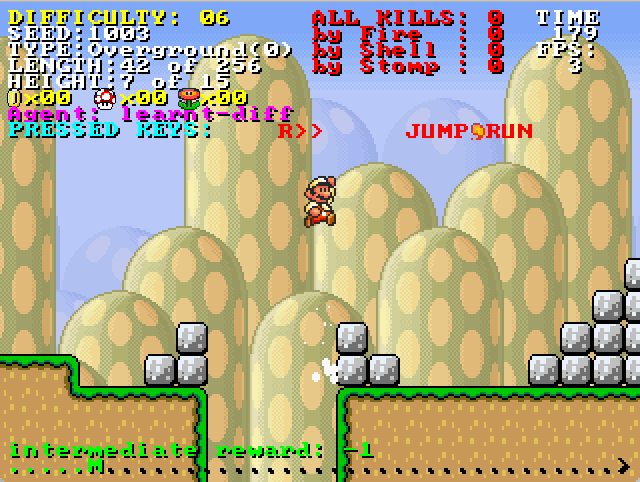
\includegraphics[width=\textwidth]{lapj4.png}
                  \caption{Rule 8}
                  \vspace*{\baselineskip}
          \end{subfigure}
          \begin{subfigure}[b]{0.49\textwidth}
                  \centering
                  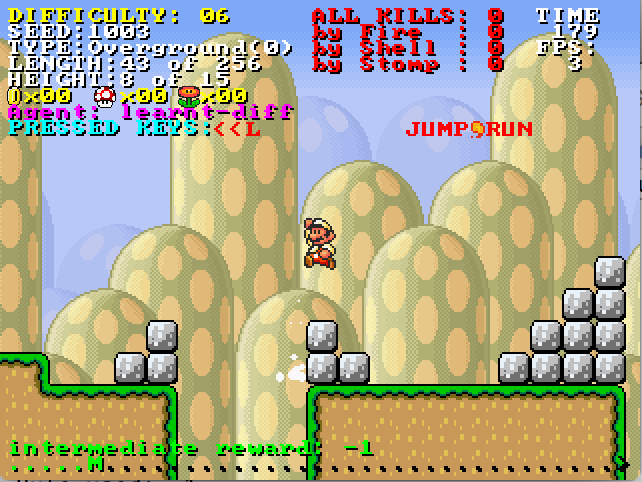
\includegraphics[width=\textwidth]{lapj5.png}
                  \caption{Rule 13}
                  \vspace*{\baselineskip}
          \end{subfigure}~
          \begin{subfigure}[b]{0.49\textwidth}
                  \centering
                  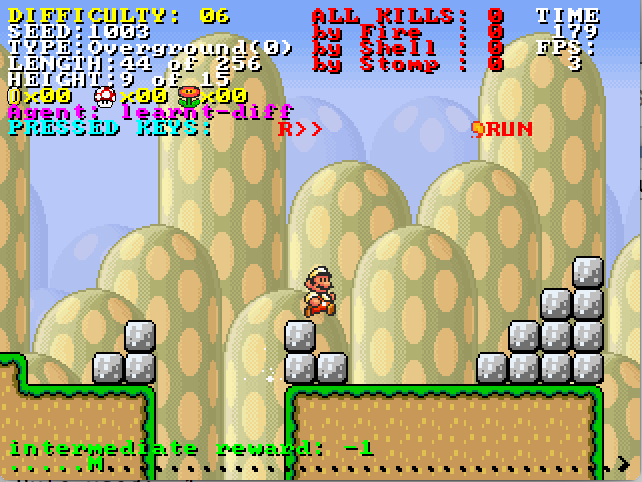
\includegraphics[width=\textwidth]{lapj6.png}
                  \caption{Default Rule}
                  \vspace*{\baselineskip}
          \end{subfigure}
    \caption{Learnt Difference agent tackling pits, without over-jumping.}\label{fig:lapj}
    \end{adjustwidth}
\end{figure}



\clearpage

\vspace*{\baselineskip}
\subsubsection*{Pits with Enemies}

\begin{table}[!h]
  \begin{adjustwidth}{-2cm}{-2cm}
  \begin{center} \scriptsize
    \begin{tabular}{| c | c | c | c | c | c | c | c || c | c | c | c |}
    \hline
    \multirow{2}{*}{\textbf{\#}} & \multicolumn{7}{c ||}{\textbf{Conditions}} & \multicolumn{4}{c |}{\textbf{Actions}} \Tstrut \\ \cline{2-12}
	& \tiny JA & \tiny OG &  \tiny EL & \tiny EUR & \tiny PA & \tiny PB & \tiny MY & \tiny Left~ & \tiny Right & \tiny Jump~ & \tiny Speed \TBstrut \\ \thickhline
	16 & 1 & 1 & 0 & & 1 & & &    T & T & T & F \\ \hline
	19 & 1 & & & 1 & 2 & 0 & 0 &    T & F & F & T \\ \hline
	- &  & & & & &  &  &    F & T & F & T \\ \hline
    \end{tabular}
  \end{center}
  \end{adjustwidth}
\end{table}

In situations when the path over a pit is blocked by an enemy the learnt difference agent displays an advanced strategy. It delays jumping over the pit until the enemy had moved away using Rule 19.

Figure \ref{fig:laepa} demonstrates the strategy. As Mario approaches a pit he first detects that one is \textbf{far} (\textbf{PA} (PitAhead) = 2), as he gets closer he detects it as \textbf{close} (\textbf{PA} = 1). If there is an enemy to his upper right (\textbf{EUR} (EnemyUpperRight) = 1) at the point he perceives the pit as \textbf{far} Rule 19 activates, which stops Mario a causes him to move left. The use of the \textbf{speed} action here, allows Mario to turn quick enough to avoid perceiving the pit as \textbf{close} and activating Rule 16. Turning and moving away from the pit allows the threat to either move away or fall into the pit (as can be seen in Figure \ref{fig:laepa}). At which point Rule 19 deactivates a Mario once again approaches the pit. If no more threats are detected he uses the pit strategy to clear the pit. The other conditions on Rule 19 also serve an important purpose: it will not occur if Mario has already started to jump over the pit. Turning left whilst already trying to clear a pit would more than likely result in Mario falling and failing the level.

The use of Rule 19 allows Mario to avoid collisions with enemies, maintaining the \textbf{fire} mode, allowing him to use fireballs. As we saw in his enemy strategy, fireballs are an important tool for clearing enemies, increasing the chances of completing a level.

This behaviour is unique to the learnt difference agent and is part of what makes it the most interesting a capable agent. 


\clearpage

\begin{figure}[t]
	\begin{adjustwidth}{-2cm}{-2cm}
    \centering
          \begin{subfigure}[b]{0.49\textwidth}
                  \centering
                  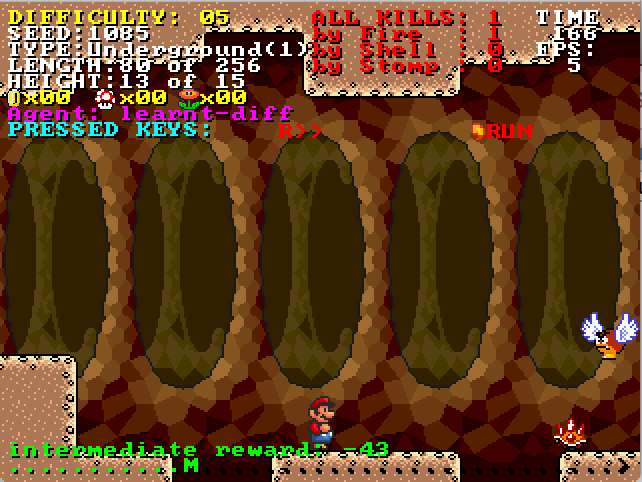
\includegraphics[width=\textwidth]{laepa1.png}
                  \caption{Default Rule}
                  \vspace*{\baselineskip}
          \end{subfigure}~
          \begin{subfigure}[b]{0.49\textwidth}
                  \centering
                  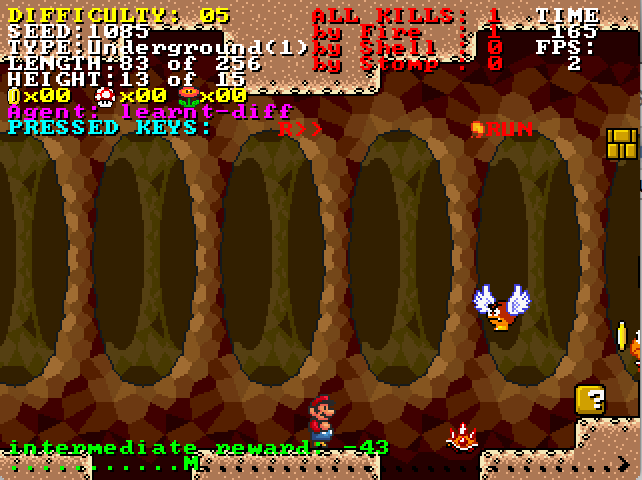
\includegraphics[width=\textwidth]{laepa2.png}
                  \caption{Default Rule}
                  \vspace*{\baselineskip}
          \end{subfigure}
          \begin{subfigure}[b]{0.49\textwidth}
                  \centering
                  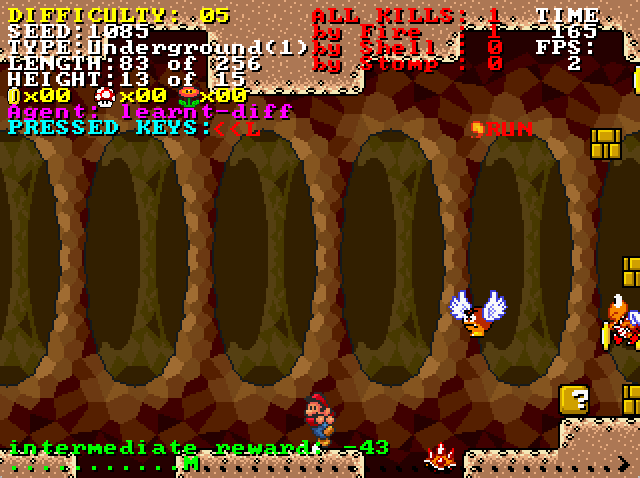
\includegraphics[width=\textwidth]{laepa3.png}
                  \caption{Rule 19}
                  \vspace*{\baselineskip}
          \end{subfigure}~
          \begin{subfigure}[b]{0.49\textwidth}
                  \centering
                  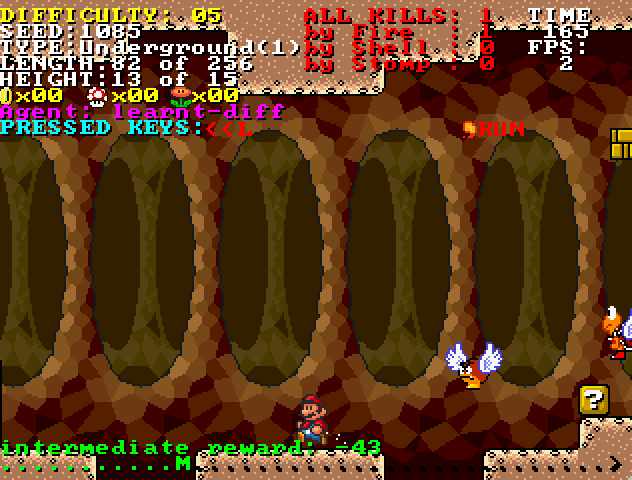
\includegraphics[width=\textwidth]{laepa4.png}
                  \caption{Rule 19}
                  \vspace*{\baselineskip}
          \end{subfigure}
          \begin{subfigure}[b]{0.49\textwidth}
                  \centering
                  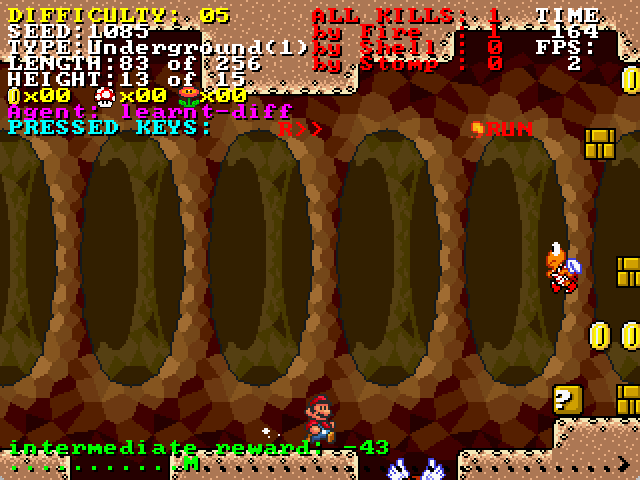
\includegraphics[width=\textwidth]{laepa5.png}
                  \caption{Default Rule}
                  \vspace*{\baselineskip}
          \end{subfigure}~
          \begin{subfigure}[b]{0.49\textwidth}
                  \centering
                  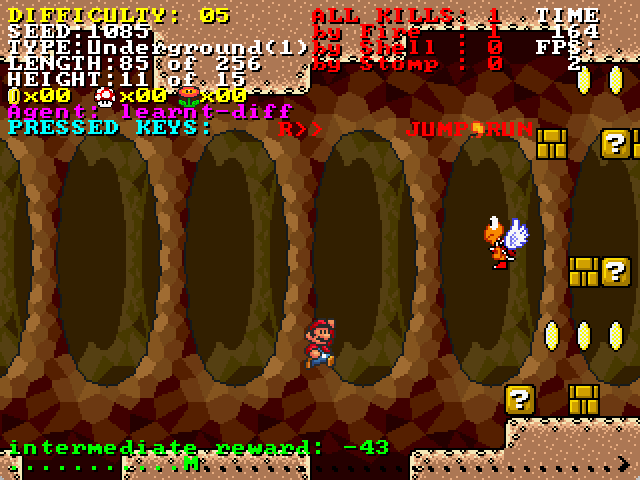
\includegraphics[width=\textwidth]{laepa6.png}
                  \caption{Rule 16}
                  \vspace*{\baselineskip}
          \end{subfigure}
    \caption{Learnt Difference agent tackling pits where enemies are blocking the jump.}\label{fig:laepa}
    \end{adjustwidth}
\end{figure}


